\chapter{Разработка метода решения задачи} \label{ch3}

% не рекомендуется использовать отдельную section <<введение>> после лета 2020 года
%\section{Введение} \label{ch3:intro}

Хорошим стилем является наличие введения к главе. Во введении может быть описана цель написания главы, а также приведена краткая структура главы. 
	
\section{Измерение инфракрасного излучения} \label{ch3:sec1}

Все объекты, температура которых превышает температуру абсолютного нуля излучают электромагнитное тепловое излучение. Согласно распределению длин волн, излучаемая энергия имеет зависимость от температуры поверхности объекта, которую можно описать законом излучения Планка:
\begin{equation} 
M(\lambda, T)=\frac{c_1 \lambda^{-5}}{\mathrm{e}^{c_2 / \lambda T}-1}
\end{equation} 
где $M(\lambda, T)$ величина излучения абсолютно черного тела. $c_1$ и $c_2$ первая и вторая константы излучения соответственно. $\lambda$ длина волны излучения и $T$ абсолютная температура черного тела. Когда $\exp \left(c_2 / \lambda T\right)>>1$, формулу Планка можно заменить следующей формулой смещения Вина:
\begin{equation} 
M_{\mathrm{b}}(\lambda, T)=c_1 \lambda^{-5} \mathrm{e}^{-c_2 / \lambda T}
\end{equation} 

Закон смещения Вина указывает на то, что чем выше температура объекта, тем короче длина волны его спектра излучения, и центральный пик смещается в сторону коротких волн. Однако излучаемая энергия, поступающая на чувствительную поверхность датчика, в реальных измерениях включает не только излучаемую энергию целевого объекта, но также энергию окружающих объектов и атмосферы. Поэтому спектральную излучательную способность поверхности целевого объекта можно выразить следующим образом:
\begin{equation} 
L_\lambda=\varepsilon_\lambda M_{\mathrm{b}}\left(\lambda, T_{\mathrm{obj}}\right)+\left(1-\alpha_\lambda\right) M_{\mathrm{b}}\left(\lambda, T_{\mathrm{sur}}\right)
\end{equation} 
где $\varepsilon_\lambda$ и $T_{\mathrm{obj}}$ излучательная способность и температура целевого объекта соответсвенно; $\varepsilon_\lambda M_b\left(\lambda, T_{\mathrm{obj}}\right)$ и $M_b(\lambda$, $T_{sur}$) это спектральная яркость целевого объекта и окружающей среды. $\alpha_\lambda$ поглощающая способность поверхности целевого объекта. $T_{\mathrm{sur}}$ температура окружающей среды.

Первый множитель в правой части уравнения (3.3) представляет собой спектральную яркость поверхности целевого объекта, а второй множитель — спектральную яркость окружающей среды, отраженную от целевого объекта. Излучение, действующее на систему измерения инфракрасного излучения, представлено на рисунке \ref{scheme}, основными источниками которого являются окружающая среда, объект и атмосфера. Это может быть выражено как:
\begin{equation} 
\begin{multlined}
E_\lambda=A_{\mathrm{obj}} d^{-2}\left[\tau_{\alpha \lambda} \varepsilon_\lambda M_{\mathrm{b}}\left(\lambda, T_{\mathrm{obj}}\right)+\tau_{\mathrm{a} \lambda}\left(1-\alpha_\lambda\right) \cdot M_{\mathrm{b}}\left(\lambda, T_{\mathrm{sur}}\right)+ \\ \varepsilon_{\alpha \lambda} M_{\mathrm{b}}\left(\lambda, T_{\mathrm{atm}}\right)\right]
\end{multlined}
\end{equation} 

\begin{figure}[ht!]
    \centering
    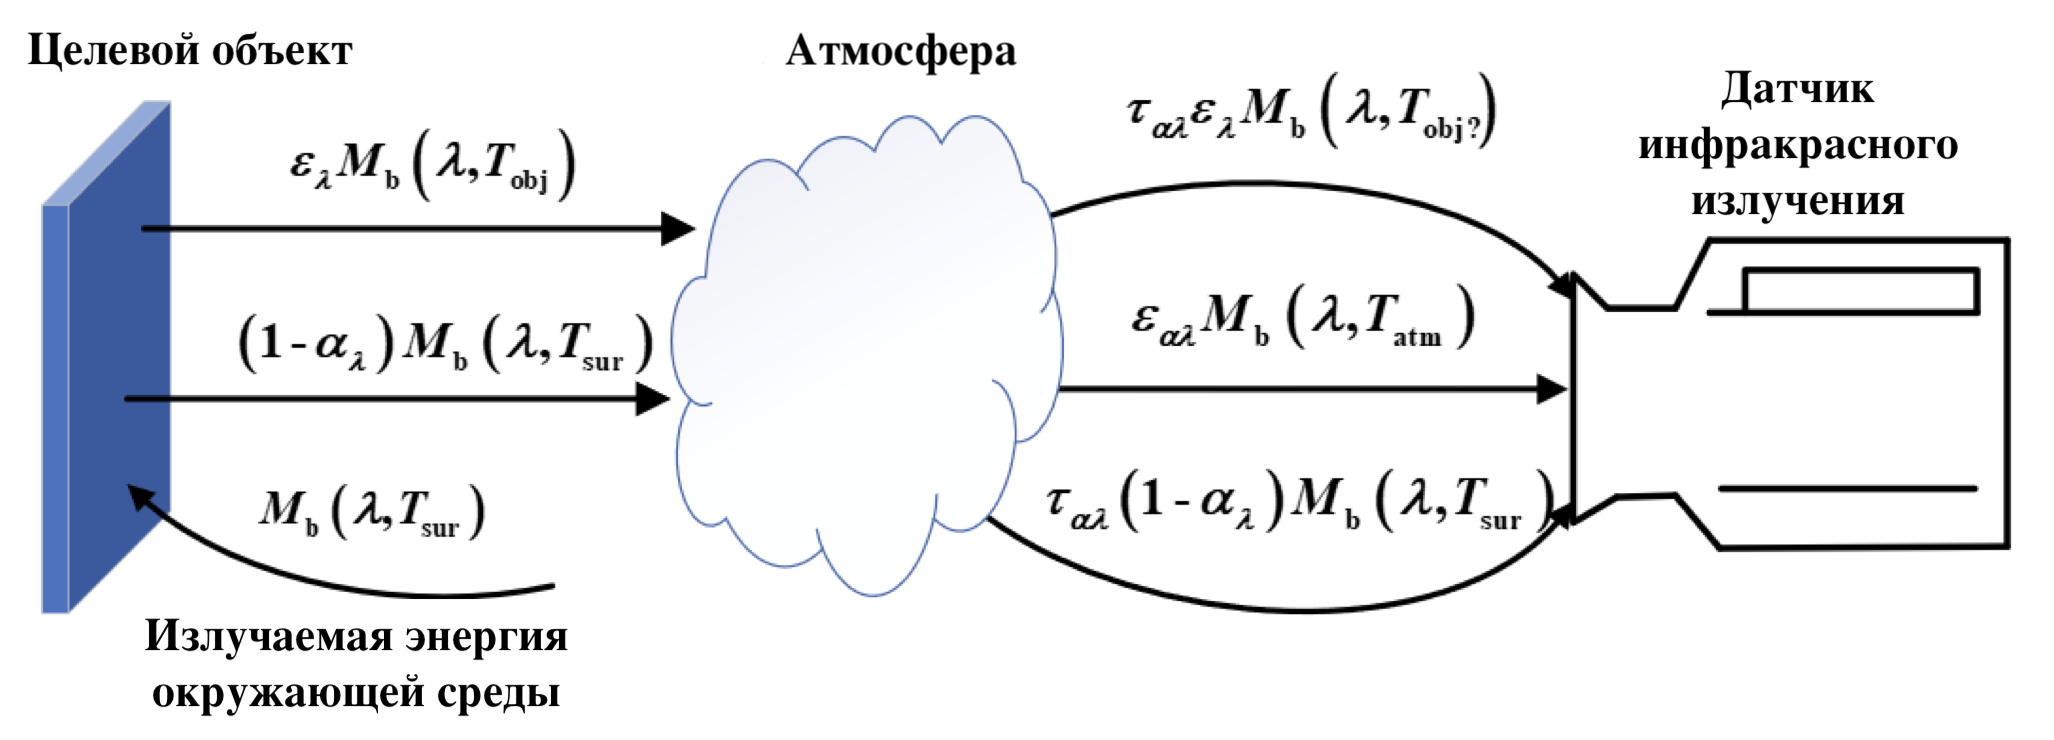
\includegraphics[width=0.8\linewidth]{my_folder/images/infr-scheme.png}
    \caption{Принципиальная схема получаемой энергии системы измерения инфракрасного излучения}
    \label{scheme}
\end{figure}
где $A_{\text{obj}}$ — видимая площадь целевого объекта, соответствующая минимальному углу тензора датчика инфракрасного изслучения, а $d$ — расстояние от целевого объекта до датчика инфракрасного излучения. В общем случае $\mathrm{A}_{\mathrm{obj}} d^{-2}$ является константой. $\tau_{\alpha \lambda}, \varepsilon_{\alpha \lambda} \mathrm{M}_{\mathrm{b}}\left(\lambda, T_{\mathrm{atm}}\right), \varepsilon_{\alpha \lambda}$ и $T_{\mathrm{atm}}$ — это спектральная пропускная способность, излучение, коэффициент излучения и температура атмосферы соответственно.

Полученная инфракрасная излучаемая энергия преобразуется датчиком в сигнал тока, то есть падающая инфракрасная излучаемая энергия интегрируется по полосе пропускания $\Delta \lambda$. Следовательно, зависимость между излучаемой энергией и током можно выразить следующим образом:
\begin{equation} 
I_0 = \int_{\Delta \lambda} A_{\mathrm{R}} R_\lambda E_\lambda \tau_{\mathrm{f}} \mathrm{d} \lambda
\end{equation} 
где $I_0$ — выходной сигнал тока датчика. $E_\lambda$ — освещенность радиации, полученная инфракрасной измерительной системой. $A_{\mathrm{R}}$ — площадь инфракрасной фокусирующей линзы. $R_\lambda$ — спектральная чувствительность инфракрасного датчика. $\tau_{\mathrm{f}}$ — пропускная способность оптической системы. Выходной ток можно преобразовать в сигнал напряжения через цепь преобразования I/V, что можно выразить следующим образом:
\begin{equation} 
\begin{multlined}
V_{\text {out }} = \int_{\Delta \lambda} R A_{\mathrm{obj}} d^{-2} A_{\mathrm{R}} \tau_f R_\lambda\left[\tau_{\alpha \lambda} \varepsilon_\lambda M_{\mathrm{b}}\left(\lambda, T_{\mathrm{obj}}\right) + \tau_{\alpha \lambda}(1 - \alpha_\lambda) M_{\mathrm{b}}\left(\lambda, T_{\text {sur}}\right) + \\ \varepsilon_{\alpha \lambda} M_{\mathrm{b}}\left(\lambda, T_{\mathrm{atm}}\right)\right] \mathrm{d} \lambda 
\end{multlined}
\end{equation}
где $R$ — нагрузка.

Уравнение (3.6) указывает, что существует множество факторов, влияющих на измерение инфракрасной температуры. На самом деле, эффективная площадь линзы, пропускная способность оптической системы и нагрузка определяются после спецификации аппаратного обеспечения системы измерения температуры. Когда $K = R A_{\mathrm{R}} \mathrm{T} \tau_{\mathrm{f}}$, уравнение (3.6) можно упростить следующим образом:
\begin{equation} 
\begin{multlined}
V_{\text {out }} = K A_{\mathrm{obj}} d^{-2} \int_{\Delta \lambda} R_\lambda\left[\tau_{\alpha \lambda} \varepsilon_\lambda \cdot M_{\mathrm{b}}\left(\lambda, T_{\mathrm{obj}}\right) + \tau_{\alpha \lambda}\left(1 - \alpha_\lambda\right) M_{\mathrm{b}}\left(\lambda, T_{\mathrm{sur}}\right) + \\\varepsilon_{\alpha \lambda} M_{\mathrm{b}}\left(\lambda, T_{\mathrm{atm}}\right)\right] \mathrm{д} \lambda
\end{multlined}
\end{equation} 

В таблице \ref{tab:equation7} представлено подробное описание переменных уравнения (3.7).

Из уравнения (3.7) видно, что точность измерений зависит от температуры окружающей среды, расстояния и угла измерения при определенной излучательной способности черного тела.

% Please add the following required packages to your document preamble:
% \usepackage{longtable}
% Note: It may be necessary to compile the document several times to get a multi-page table to line up properly
\begin{longtable}{|l|l|l|l|}
\caption{Описание переменных уравнения (3.7)}
\label{tab:equation7}\\
\hline
\multicolumn{1}{|c|}{Переменная}                & \multicolumn{1}{c|}{Описание}                                                                                                                                                  & \multicolumn{1}{c|}{Источник значения}                                                                                      & \multicolumn{1}{c|}{\begin{tabular}[c]{@{}c@{}}Единица \\ измерения\end{tabular}}                                           \\ \hline
\endhead
%
\( V_{\text{out}} \)                            & \begin{tabular}[c]{@{}l@{}}Выходное напряжение \\ на инфракрасном датчике\end{tabular}                                                                                         & \begin{tabular}[c]{@{}l@{}}Результат \\ измерений\end{tabular}                                                              & Вольт (V)                                                                                                                   \\ \hline
\( K \)                                         & \begin{tabular}[c]{@{}l@{}}Константа, определяющая \\ параметры оптической \\ системы инфракрасного \\ датчика: площадь линзы, \\ пропускная способность \\ линзы\end{tabular} & \begin{tabular}[c]{@{}l@{}}Задается \\ характеристиками \\ инфракрасного \\ детектора\end{tabular}                          & \begin{tabular}[c]{@{}l@{}}Безразмерная\\ величина\end{tabular}                                                             \\ \hline
\( A_{\text{obj}} \)                            & \begin{tabular}[c]{@{}l@{}}Видимая площадь \\ наблюдаемого \\ объекта\end{tabular}                                                                                             & \begin{tabular}[c]{@{}l@{}}Определяется \\ геометрией \\ объекта и \\ углом зрения \\ инфракрасного \\ датчика\end{tabular} & \begin{tabular}[c]{@{}l@{}}Квадратные \\ метры (\( \text{м}^2 \) )\end{tabular}                                             \\ \hline
\( d \)                                         & \begin{tabular}[c]{@{}l@{}}Расстояние от \\ наблюдаемого \\ объекта до \\ инфракрасного \\ датчика\end{tabular}                                                                & \begin{tabular}[c]{@{}l@{}}Измеряется в \\ экспериментальных \\ условиях\end{tabular}                                       & Метры (м)                                                                                                                   \\ \hline
\( \Delta \lambda \)                            & \begin{tabular}[c]{@{}l@{}}Спектральный \\ диапазон измерений\end{tabular}                                                                                                     & \begin{tabular}[c]{@{}l@{}}Задается \\ характеристиками \\ инфракрасного \\ датчика\end{tabular}                            & \begin{tabular}[c]{@{}l@{}}Микрометры \\ ( \( \mu \) m)\end{tabular}                                                        \\ \hline
\( R_\lambda \)                                 & \begin{tabular}[c]{@{}l@{}}Спектральная \\ чувствительность \\ инфракрасного \\ датчика\end{tabular}                                                                           & \begin{tabular}[c]{@{}l@{}}Задается \\ характеристиками \\ инфракрасного \\ датчика\end{tabular}                            & \begin{tabular}[c]{@{}l@{}}Безразмерная\\ величина\end{tabular}                                                             \\ \hline
\( \tau_{\alpha \lambda} \)                     & \begin{tabular}[c]{@{}l@{}}Спектральная \\ пропускная \\ способность \\ атмосферы\end{tabular}                                                                                 & \begin{tabular}[c]{@{}l@{}}Табличные или \\ экспериментальные\\ данные\end{tabular}                                         & \begin{tabular}[c]{@{}l@{}}Безразмерная\\ величина\end{tabular}                                                             \\ \hline
\( \varepsilon_\lambda \)                       & \begin{tabular}[c]{@{}l@{}}Излучательная \\ способность объекта\end{tabular}                                                                                                   & Табличные данные                                                                                                            & \begin{tabular}[c]{@{}l@{}}Безразмерная\\ величина\end{tabular}                                                             \\ \hline
\( M_{\mathrm{b}}(\lambda, T_{\mathrm{obj}}) \) & \begin{tabular}[c]{@{}l@{}}Спектральная плотность \\ излучения объекта при \\ температуре \( T_{\mathrm{obj}} \)\end{tabular}                                                  & \begin{tabular}[c]{@{}l@{}}Вычисляется по \\ закону Планка\end{tabular}                                                     & \begin{tabular}[c]{@{}l@{}}Ватты на \\ квадратный \\ метр на \\ микрометр \\ (Вт/\( \text{м}^2 \)/\( \mu \) м)\end{tabular} \\ \hline
\( M_{\mathrm{b}}(\lambda, T_{\mathrm{sur}}) \) & \begin{tabular}[c]{@{}l@{}}Спектральная плотность \\ излучения окружающей \\ среды при \\ температуре \( T_{\mathrm{sur}} \)\end{tabular}                                      & \begin{tabular}[c]{@{}l@{}}Вычисляется по \\ закону Планка\end{tabular}                                                     & \begin{tabular}[c]{@{}l@{}}Ватты на \\ квадратный \\ метр на \\ микрометр \\ (Вт/\( \text{м}^2 \)/\( \mu \) м)\end{tabular} \\ \hline
\( \tau_{\alpha \lambda}(1-\alpha_\lambda) \)   & \begin{tabular}[c]{@{}l@{}}Фактор отражения \\ излучения \\ окружающей среды\end{tabular}                                                                                      & \begin{tabular}[c]{@{}l@{}}Табличные или \\ экспериментальные\\ данные\end{tabular}                                         & \begin{tabular}[c]{@{}l@{}}Безразмерная\\ величина\end{tabular}                                                             \\ \hline
\( M_{\mathrm{b}}(\lambda, T_{\mathrm{atm}}) \) & \begin{tabular}[c]{@{}l@{}}Спектральная плотность \\ излучения атмосферы \\ при температуре \( T_{\mathrm{atm}} \)\end{tabular}                                                & \begin{tabular}[c]{@{}l@{}}Вычисляется по \\ закону Планка\end{tabular}                                                     & \begin{tabular}[c]{@{}l@{}}Ватты на \\ квадратный \\ метр на \\ микрометр \\ (Вт/\( \text{м}^2 \)/\( \mu \) м)\end{tabular} \\ \hline
\( \varepsilon_{\alpha \lambda} \)              & \begin{tabular}[c]{@{}l@{}}Спектральная излучательная \\ способность атмосферы\end{tabular}                                                                                    & \begin{tabular}[c]{@{}l@{}}Табличные или \\ экспериментальные\\ данные\end{tabular}                                         & \begin{tabular}[c]{@{}l@{}}Безразмерная\\ величина\end{tabular}                                                             \\ \hline
\end{longtable}

\subsection{Погрешности измерения инфракрасного излучения}
В практическом применении при проведении измерения инфракрасного излучения существенное значение имеет выявление и устранение систематических и случайных погрешностей, оказывающих влияние на результаты измерения.

Систематические погрешности заключены в конструкции измерительного прибора, а также зависят от его выбора в соответствии с требованиями к совершенству измерения (разрешающей способности, поля зрения и т.п.).

Случайными погрешностями, возникающими при проведении измерения инфракрасного излучения, могут являться: 
\begin{itemize}
    \item коэффициент излучения материала;
    \item солнечная радиация;
    \item расстояние до объекта;
    \item тепловое отражение и т.п.
\end{itemize}

\subsection{Коэффициент доверия}
Для вычисления уровня доверия к результатам измерения на основе различных параметров, можно выбрать ключевые изменяемые параметры из формулы (3.7). 

Основными параметрами, влияющими на измерения, являются:

\begin{itemize}
    \item расстояние до объекта (\(d\));
    \item угол наблюдения (\(\theta\));
    \item температура атмосферы (\(T_{\text{atm}}\));
    \item спектральная пропускная способность атмосферы (\(\tau_{\alpha \lambda}\));
    \item спектральная излучательная способность объекта (\(\varepsilon_\lambda\))
\end{itemize}

\textbf{Формула для вычисления уровня доверия}

Предположим, что каждый параметр влияет на уровень доверия линейно и независимо. Можно назначить каждому параметру весовой коэффициент, отражающий его относительное влияние на общий уровень доверия.
\begin{equation}
D = w_d \cdot f_d(d) + w_\theta \cdot f_\theta(\theta) + w_{T_{\text{atm}}} \cdot f_{T_{\text{atm}}}(T_{\text{atm}}) + w_{\tau_{\alpha \lambda}} \cdot f_{\tau_{\alpha \lambda}}(\tau_{\alpha \lambda}) + w_{\varepsilon_\lambda} \cdot f_{\varepsilon_\lambda}(\varepsilon_\lambda)
\end{equation}

Где:
\begin{itemize}
    \item \(d\) — расстояние до объекта,
    \item \(\theta\) — угол наблюдения,
    \item \(T_{\text{atm}}\) — температура атмосферы,
    \item \(\tau_{\alpha \lambda}\) — спектральная пропускная способность атмосферы,
    \item \(\varepsilon_\lambda\) — излучательная способность объекта
\end{itemize}

\textbf{Функции и веса}

Для каждого параметра определим нормированные функции \(f_i\), принимающие значения от 0 до 1, и весовые коэффициенты \(w_i\), сумма которых равна 1.

1. Расстояние до объекта (\(d\)):
   \[ f_d(d) = \frac{1}{1 + k_d \cdot d} \]
   Где \(k_d\) — коэффициент, определяющий, как быстро снижается уровень доверия с увеличением расстояния.

2. Угол наблюдения (\(\theta\)):
   \[ f_\theta(\theta) = \cos(\theta) \]
   
   Так как по закону Ламберта интенсивность радиации пропорциональна косинусу угла наблюдения.

3. Температура атмосферы (\(T_{\text{atm}}\)):
   \[ f_{T_{\text{atm}}}(T_{\text{atm}}) = 1 - \left| \frac{T_{\text{atm}} - T_{\text{opt}}}{T_{\text{max}} - T_{\text{min}}} \right| \]
   Где \(T_{\text{opt}}\) — оптимальная температура для измерений, \(T_{\text{max}}\) и \(T_{\text{min}}\) — максимальная и минимальная температуры, соответственно.

4. Спектральная пропускная способность атмосферы (\(\tau_{\alpha \lambda}\)):
   \[ f_{\tau_{\alpha \lambda}}(\tau_{\alpha \lambda}) = \tau_{\alpha \lambda} \]
   
   Прямо пропорциональна пропускной способности атмосферы.

5. Излучательная способность объекта (\(\varepsilon_\lambda\)):
   \[ f_{\varepsilon_\lambda}(\varepsilon_\lambda) = \varepsilon_\lambda \]
   
   Прямо пропорциональна излучательной способности объекта.


\textbf{Пример весовых коэффициентов}

Пусть весовые коэффициенты распределены следующим образом:
\[w_d = 0.3\] 
\[w_\theta = 0.25\]
\[w_{T_{\text{atm}}} = 0.2\]
\[w_{\tau_{\alpha \lambda}} = 0.15\]
\[w_{\varepsilon_\lambda} = 0.1\]

С учетом вышеуказанных весов и функций, получаем формулу:
\[ D = 0.3 \cdot \frac{1}{1 + k_d \cdot d} + 0.25 \cdot \cos(\theta) + 0.2 \cdot \left(1 - \left| \frac{T_{\text{atm}} - T_{\text{opt}}}{T_{\text{max}} - T_{\text{min}}} \right| \right) + 0.15 \cdot \tau_{\alpha \lambda} + 0.1 \cdot \varepsilon_\lambda \]


\textbf{Пример набора параметров и расчет уровня доверия}

Пусть:
\[d = 20 \, \text{м}\]
\[\theta = 30^\circ\]
\[T_{\text{atm}} = 25 \, \text{°C}\] 
\[T_{\text{opt}} = 20 \, \text{°C}\]
\[T_{\text{max}} = 35 \, \text{°C}\] 
\[T_{\text{min}} = 5 \, \text{°C}\]
\[\tau_{\alpha \lambda} = 0.85\]
\[\varepsilon_\lambda = 0.9\]

Тогда:
\[f_d(20) = \frac{1}{1 + k_d \cdot 20} \text{, предположим } k_d = 0.05 \text{, тогда } f_d(20) = \frac{1}{1 + 1} = 0.5 \]

\[f_\theta(30^\circ) = \cos(30^\circ) = \sqrt{3}/2 \approx 0.866\] 

\[f_{T_{\text{atm}}}(25) = 1 - \left| \frac{25 - 20}{35 - 5} \right| = 1 - \frac{5}{30} = 0.833\]

\[f_{\tau_{\alpha \lambda}}(0.85) = 0.85\] 

\[f_{\varepsilon_\lambda}(0.9) = 0.9\] 

Подставляя значения в формулу:

\[ D = 0.3 \cdot 0.5 + 0.25 \cdot 0.866 + 0.2 \cdot 0.833 + 0.15 \cdot 0.85 + 0.1 \cdot 0.9 \]
\[ D = 0.15 + 0.2165 + 0.1666 + 0.1275 + 0.09 \]
\[ D = 0.7506 \]

\section{Использование методов машинного обучения}
Во многих известных оптических системах беспилотных летательных аппаратов используются алгоритмы распознавания и селекции объектов. В случае если целевой объект находится, например, высоко в воздухе, его детектирование можно осуществить оптическим контрастированием из-за хорошей отличимости объекта от окружающего фона (неба) или в инфракрасном диапазоне спектра из-за большой разности температур объекта и окружающей среды. Однако данные методы работают не столь эффективно для оптических устройств беспилотных летательных аппаратов, сканирующих Земную поверхность, т.к. сцены в этом случае становятся многообъектными и автоматическое обнаружение нужного объекта будет затруднено всевозможными помехами. В данном случае целесообразно рассмотреть методы распознавания образов с помощью алгоритмов машинного обучения и технологии искусственного интеллекта.

При построении систем управления движущимися объектами различного назначения особое внимание уделяется выбору типа и набора бортовых сенсорных устройств и их характеристик, обеспечивающих получение достоверной информации о состоянии окружающей среды и, как следствие, эффективное решение поставленной задачи управления в различных условиях применения. Большое распространение получили оптико-электронные системы для вывода на экран оператора видеоизображения, полученного при помощи тепловизионной (ТПВ) и телевизионной (ТВ) камер (рис. \ref{teplovision}) .
\begin{figure}[ht!]
    \centering
    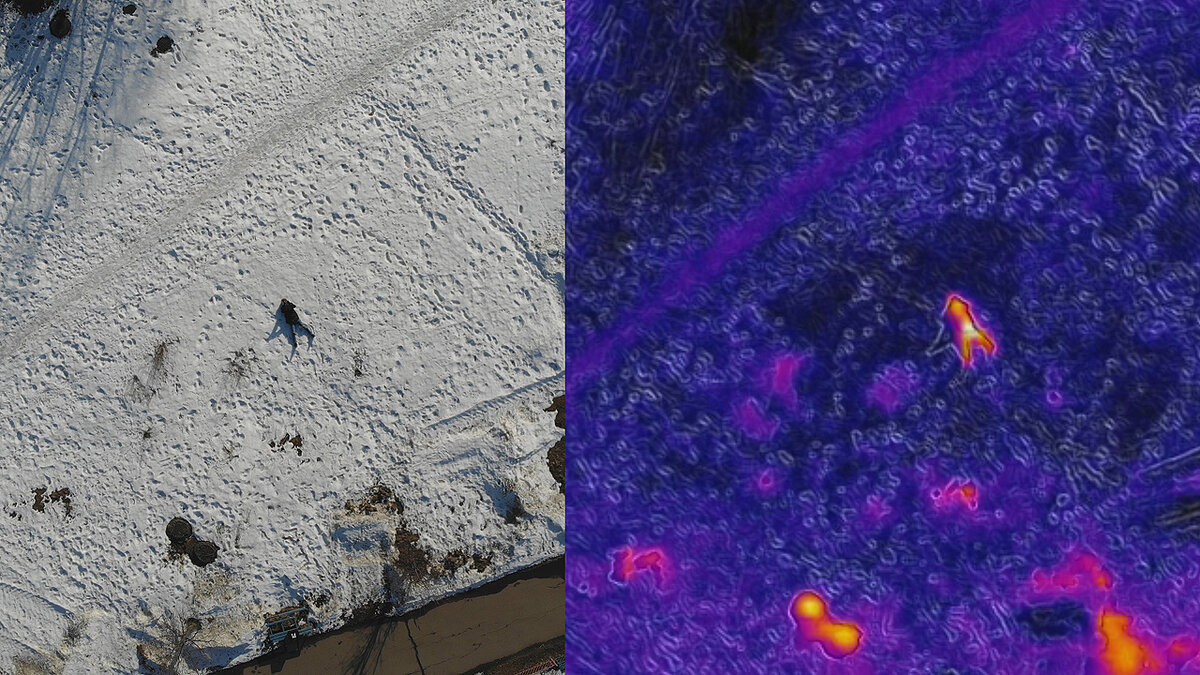
\includegraphics[width=0.8\linewidth]{my_folder/images/teplovision.jpeg}
    \caption{Пример съемки на Mavic 2 Enterprise Dual с высоты 40 метров}
    \label{teplovision}
\end{figure}

ТВ приборы обладают одним существенным недостатком: наличие дождя, снега, тумана и т.д. затрудняет видение в таких условиях либо вовсе исключает такую возможность. Проблема обеспечения видения в таких экстремальных условиях может быть решена с помощью тепловизионных приборов. Тепловизионные приборы также обладают рядом недостатков. Из-за своей низкой пространственной разрешающей способности они не выявляют мелких подробностей наблюдаемого пространства. Но самое главное – тепловизионные приборы позволяют видеть только те объекты, температура которых отличается от температуры окружающего фона, т.е. при наличии температурного контраста.

Полезными признаками для телевизионных изображений являются \cite{optical-prisnaki}:
\begin{itemize}
    \item форма,
    \item размеры,
    \item текстура,
    \item внутренняя структура объектов,
    \item окружение.
\end{itemize}

Полезными признаками для тепловизионных изображений являются:
\begin{itemize}
    \item форма,
    \item  максимальное/минимальное значение эмиссии,
    \item  количество и расположение горячих пятен,
    \item окружение (среда). 
\end{itemize}

Распознавание трехмерных объектов по их двумерным изображениям стало в последнее время одной из важнейших задач анализа сцен и компьютерного зрения. Под объектом понимается не только цифровое представление локального фрагмента двумерной сцены, но и некоторое его приближенное описание, в виде набора характерных свойств (признаков). Признаки – это измерения, используемые для классификации объектов [\cite{rasposnavanie}].

При реализации задачи локализации парадигма решения может формулироваться следующим образом: на основе априорной информации о рассматриваемой сцене (участке Земной поверхности) и апостериорной информации о той же сцене, полученной в процессе полета, сопоставляются текущее и эталонное изображения с последующей локализацией на текущем изображении заданных объектов сцены и определением значений текущих координат этих объектов в целях формирования сигналов управления движением летательного аппарата \cite{insarov}.

\section{Анализ методов машинного обучения}
\subsection{Сверточные нейронные сети}
Сверточные нейронные сети представляют собой класс искусственных нейронных сетей, специально разработанных для обработки и анализа изображений. Их архитектура и механизмы позволяют эффективно распознавать сложные паттерны в визуальных данных, что делает их незаменимыми в различных областях компьютерного зрения.

Основными компонентами являются сверточные слои, слои объединения (пулинга) и полностью связанные слои.
\begin{enumerate}
    \item Сверточные слои выполняют операцию свертки, применяя фильтры или ядра к исходному изображению. Фильтры помогают выделять различные признаки, такие как края, углы и текстуры. Каждый фильтр генерирует карту признаков, которая подчеркивает определенные аспекты входного изображения.
    \item Слои объединения пулинга уменьшают размерность карт признаков, что снижает вычислительную нагрузку и вероятность переобучения. Наиболее распространенными методами объединения являются максимальный пулинг (максимальное значение в каждом подокне) и средний пулинг (среднее значение в каждом подокне).
    \item Полностью связанные слои находятся в конце сети и служат для окончательной классификации. Они соединяют все нейроны предыдущего слоя с каждым нейроном текущего слоя, позволяя учитывать все выделенные ранее признаки.
\end{enumerate}

Сверточные нейронные сети обладают рядом преимуществ, делающих их эффективными для обработки изображений. В первую очередь свойства сверточных слоев позволяют учитывать локальные пространственные отношения между пикселями, что важно для распознавания объектов. Использование методов, таких как нормализация локальных откликов и Dropout, помогает уменьшить вероятность переобучения. Также, сверточные нейронные сети могут эффективно обучаться на больших объемах данных благодаря использованию графических процессоров (\textit{GPU}), что значительно ускоряет процесс обучения.

Сверточные нейронные сети широко применяются для решения различных задач в области классификации изображений. Например, используются для идентификации и верификации лиц на изображениях и в видео; помогают в анализе медицинских изображений, таких как рентгеновские снимки и МРТ, для обнаружения патологий; используются для распознавания объектов и ситуаций на дорогах, что необходимо для безопасного управления транспортом.

Современные исследования в области сверточных нейронных сетей направлены на улучшение архитектуры и алгоритмов обучения. Разрабатываются новые методы нормализации и регуляризации, такие как \textit{Batch Normalization} и новые типы нелинейностей (например, \textit{ReLU}). Ведутся работы по созданию более эффективных моделей, которые требуют меньше вычислительных ресурсов и могут работать в реальном времени.

\subsection{Aggregate Channel Features}
Метод \textit{ACF (Aggregate Channel Features)} является инновационным подходом в области распознавания лиц, который направлен на решение проблем, связанных с большими изменениями внешнего вида лиц в естественных условиях. Данный метод опирается на концепцию каналов изображения, расширяя их до различных типов, таких как градиенты и гистограммы ориентированных градиентов, что позволяет кодировать разнообразную признаками информацию в простой форме.

Исторически, одним из самых влиятельных подходов к распознаванию лиц был метод \textit{Viola-Jones}, который использует прямоугольные признаки, похожие на признаки Хаара, и обучает классификатор с помощью алгоритма \textit{Adaboost}. Этот метод достиг значительных успехов в распознавании лиц в реальном времени, но его производительность все еще оставалась ограниченной из-за большой изменчивости внешнего вида лиц в неконтролируемых условиях. Для преодоления этого ограничения метод \textit{ACF} использует расширенные каналы изображения, такие как градиенты и гистограммы ориентированных градиентов, что позволяет более эффективно кодировать информацию о лицах.

Метод \textit{ACF} включает в себя несколько ключевых аспектов. Во-первых, он использует расширенные каналы изображения для кодирования разнообразной информации. Например, цветовые каналы в пространстве \textit{LUV}, каналы градиентной величины и гистограммы градиентов в \textit{RGB} пространстве показывают наилучшие результаты при распознавании лиц. Эти каналы обеспечивают богатую репрезентационную способность, что особенно важно для обработки лиц с различными выражениями и позами.

Во-вторых, метод \textit{ACF} предусматривает мультискейлинг представления признаков, что позволяет еще больше обогатить репрезентацию. В оригинальной версии метода все признаки имели одинаковый масштаб, но эксперименты показали, что мультискейлинг улучшает производительность. Это достигается за счет изменения масштаба восприятия, локального масштаба и масштаба интеграции признаков.

Третьим важным аспектом является подход к мультивидовому распознаванию лиц, который использует повторную ранжировку оценок и корректировку обнаружений. Это помогает эффективно справляться с различными позами лиц и улучшает точность локализации лиц в изображениях. В результате, метод \textit{ACF} демонстрирует конкурентоспособные результаты на сложных наборах данных, таких как \textit{AFW} и \textit{FDDB}, показывая высокую точность и скорость распознавания (до 42 кадров в секунду на изображениях \textit{VGA}).

Метод \textit{ACF} значительно улучшает производительность распознавания лиц благодаря тщательному исследованию и оптимизации различных параметров признаков. Он предлагает более быструю и точную альтернативу традиционным методам распознавания лиц, обеспечивая богатую репрезентацию и высокую эффективность вычислений.

\section{Выводы} \label{ch3:conclusion}

Текст выводов по главе \thechapter.


%% Вспомогательные команды - Additional commands
%
%\newpage % принудительное начало с новой страницы, использовать только в конце раздела
%\clearpage % осуществляется пакетом <<placeins>> в пределах секций
%\newpage\leavevmode\thispagestyle{empty}\newpage % 100 % начало новой страницы